% Created by tikzDevice version 0.12.3 on 2020-01-08 08:04:11
% !TEX encoding = UTF-8 Unicode
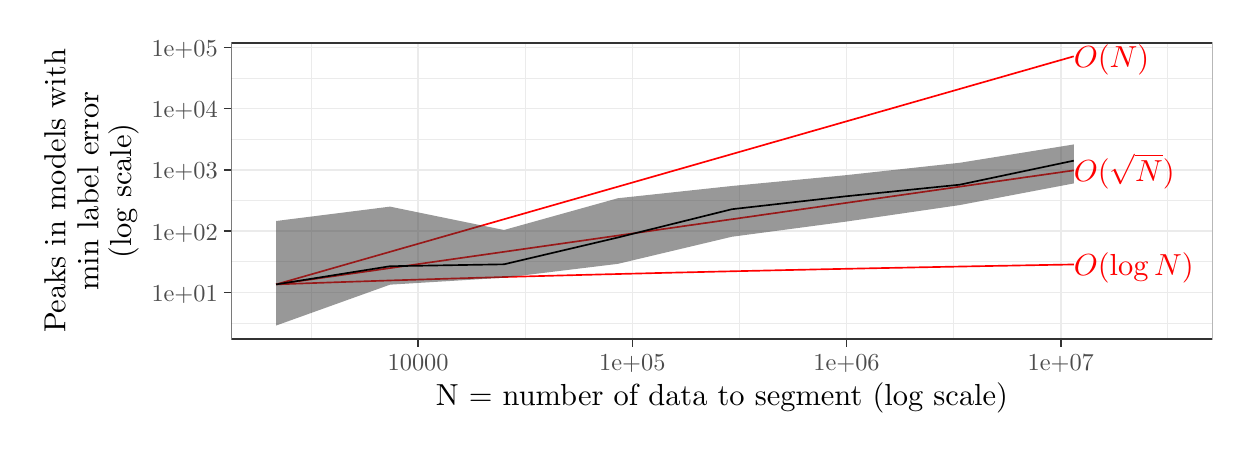
\begin{tikzpicture}[x=1pt,y=1pt]
\definecolor{fillColor}{RGB}{255,255,255}
\path[use as bounding box,fill=fillColor,fill opacity=0.00] (0,0) rectangle (433.62,144.54);
\begin{scope}
\path[clip] (  0.00,  0.00) rectangle (433.62,144.54);
\definecolor{drawColor}{RGB}{255,255,255}
\definecolor{fillColor}{RGB}{255,255,255}

\path[draw=drawColor,line width= 0.6pt,line join=round,line cap=round,fill=fillColor] (  0.00,  0.00) rectangle (433.62,144.54);
\end{scope}
\begin{scope}
\path[clip] ( 73.65, 32.04) rectangle (428.12,139.04);
\definecolor{fillColor}{RGB}{255,255,255}

\path[fill=fillColor] ( 73.65, 32.04) rectangle (428.12,139.04);
\definecolor{drawColor}{gray}{0.92}

\path[draw=drawColor,line width= 0.3pt,line join=round] ( 73.65, 37.82) --
	(428.12, 37.82);

\path[draw=drawColor,line width= 0.3pt,line join=round] ( 73.65, 59.95) --
	(428.12, 59.95);

\path[draw=drawColor,line width= 0.3pt,line join=round] ( 73.65, 82.08) --
	(428.12, 82.08);

\path[draw=drawColor,line width= 0.3pt,line join=round] ( 73.65,104.21) --
	(428.12,104.21);

\path[draw=drawColor,line width= 0.3pt,line join=round] ( 73.65,126.34) --
	(428.12,126.34);

\path[draw=drawColor,line width= 0.3pt,line join=round] (102.37, 32.04) --
	(102.37,139.04);

\path[draw=drawColor,line width= 0.3pt,line join=round] (179.78, 32.04) --
	(179.78,139.04);

\path[draw=drawColor,line width= 0.3pt,line join=round] (257.19, 32.04) --
	(257.19,139.04);

\path[draw=drawColor,line width= 0.3pt,line join=round] (334.60, 32.04) --
	(334.60,139.04);

\path[draw=drawColor,line width= 0.3pt,line join=round] (412.01, 32.04) --
	(412.01,139.04);

\path[draw=drawColor,line width= 0.6pt,line join=round] ( 73.65, 48.88) --
	(428.12, 48.88);

\path[draw=drawColor,line width= 0.6pt,line join=round] ( 73.65, 71.02) --
	(428.12, 71.02);

\path[draw=drawColor,line width= 0.6pt,line join=round] ( 73.65, 93.15) --
	(428.12, 93.15);

\path[draw=drawColor,line width= 0.6pt,line join=round] ( 73.65,115.28) --
	(428.12,115.28);

\path[draw=drawColor,line width= 0.6pt,line join=round] ( 73.65,137.41) --
	(428.12,137.41);

\path[draw=drawColor,line width= 0.6pt,line join=round] (141.08, 32.04) --
	(141.08,139.04);

\path[draw=drawColor,line width= 0.6pt,line join=round] (218.49, 32.04) --
	(218.49,139.04);

\path[draw=drawColor,line width= 0.6pt,line join=round] (295.89, 32.04) --
	(295.89,139.04);

\path[draw=drawColor,line width= 0.6pt,line join=round] (373.30, 32.04) --
	(373.30,139.04);
\definecolor{drawColor}{RGB}{255,0,0}

\path[draw=drawColor,line width= 0.6pt,line join=round] ( 89.76, 51.77) --
	( 92.67, 51.88) --
	( 95.58, 51.98) --
	( 98.49, 52.09) --
	(101.41, 52.19) --
	(104.32, 52.30) --
	(107.23, 52.40) --
	(110.14, 52.50) --
	(113.05, 52.60) --
	(115.96, 52.70) --
	(118.87, 52.80) --
	(121.79, 52.89) --
	(124.70, 52.99) --
	(127.61, 53.08) --
	(130.52, 53.18) --
	(133.43, 53.27) --
	(136.34, 53.36) --
	(139.26, 53.45) --
	(142.17, 53.54) --
	(145.08, 53.63) --
	(147.99, 53.72) --
	(150.90, 53.81) --
	(153.81, 53.90) --
	(156.72, 53.98) --
	(159.64, 54.07) --
	(162.55, 54.16) --
	(165.46, 54.24) --
	(168.37, 54.32) --
	(171.28, 54.41) --
	(174.19, 54.49) --
	(177.11, 54.57) --
	(180.02, 54.65) --
	(182.93, 54.73) --
	(185.84, 54.81) --
	(188.75, 54.89) --
	(191.66, 54.97) --
	(194.57, 55.04) --
	(197.49, 55.12) --
	(200.40, 55.20) --
	(203.31, 55.27) --
	(206.22, 55.35) --
	(209.13, 55.42) --
	(212.04, 55.49) --
	(214.96, 55.57) --
	(217.87, 55.64) --
	(220.78, 55.71) --
	(223.69, 55.78) --
	(226.60, 55.86) --
	(229.51, 55.93) --
	(232.42, 56.00) --
	(235.34, 56.07) --
	(238.25, 56.13) --
	(241.16, 56.20) --
	(244.07, 56.27) --
	(246.98, 56.34) --
	(249.89, 56.41) --
	(252.81, 56.47) --
	(255.72, 56.54) --
	(258.63, 56.60) --
	(261.54, 56.67) --
	(264.45, 56.73) --
	(267.36, 56.80) --
	(270.27, 56.86) --
	(273.19, 56.93) --
	(276.10, 56.99) --
	(279.01, 57.05) --
	(281.92, 57.11) --
	(284.83, 57.18) --
	(287.74, 57.24) --
	(290.66, 57.30) --
	(293.57, 57.36) --
	(296.48, 57.42) --
	(299.39, 57.48) --
	(302.30, 57.54) --
	(305.21, 57.60) --
	(308.12, 57.66) --
	(311.04, 57.72) --
	(313.95, 57.77) --
	(316.86, 57.83) --
	(319.77, 57.89) --
	(322.68, 57.95) --
	(325.59, 58.00) --
	(328.51, 58.06) --
	(331.42, 58.12) --
	(334.33, 58.17) --
	(337.24, 58.23) --
	(340.15, 58.28) --
	(343.06, 58.34) --
	(345.97, 58.39) --
	(348.89, 58.45) --
	(351.80, 58.50) --
	(354.71, 58.55) --
	(357.62, 58.61) --
	(360.53, 58.66) --
	(363.44, 58.71) --
	(366.36, 58.77) --
	(369.27, 58.82) --
	(372.18, 58.87) --
	(375.09, 58.92) --
	(378.00, 58.97);

\path[draw=drawColor,line width= 0.6pt,line join=round] ( 89.76, 51.77) --
	( 92.67, 52.19) --
	( 95.58, 52.60) --
	( 98.49, 53.02) --
	(101.41, 53.43) --
	(104.32, 53.85) --
	(107.23, 54.27) --
	(110.14, 54.68) --
	(113.05, 55.10) --
	(115.96, 55.52) --
	(118.87, 55.93) --
	(121.79, 56.35) --
	(124.70, 56.76) --
	(127.61, 57.18) --
	(130.52, 57.60) --
	(133.43, 58.01) --
	(136.34, 58.43) --
	(139.26, 58.84) --
	(142.17, 59.26) --
	(145.08, 59.68) --
	(147.99, 60.09) --
	(150.90, 60.51) --
	(153.81, 60.93) --
	(156.72, 61.34) --
	(159.64, 61.76) --
	(162.55, 62.17) --
	(165.46, 62.59) --
	(168.37, 63.01) --
	(171.28, 63.42) --
	(174.19, 63.84) --
	(177.11, 64.26) --
	(180.02, 64.67) --
	(182.93, 65.09) --
	(185.84, 65.50) --
	(188.75, 65.92) --
	(191.66, 66.34) --
	(194.57, 66.75) --
	(197.49, 67.17) --
	(200.40, 67.58) --
	(203.31, 68.00) --
	(206.22, 68.42) --
	(209.13, 68.83) --
	(212.04, 69.25) --
	(214.96, 69.67) --
	(217.87, 70.08) --
	(220.78, 70.50) --
	(223.69, 70.91) --
	(226.60, 71.33) --
	(229.51, 71.75) --
	(232.42, 72.16) --
	(235.34, 72.58) --
	(238.25, 73.00) --
	(241.16, 73.41) --
	(244.07, 73.83) --
	(246.98, 74.24) --
	(249.89, 74.66) --
	(252.81, 75.08) --
	(255.72, 75.49) --
	(258.63, 75.91) --
	(261.54, 76.32) --
	(264.45, 76.74) --
	(267.36, 77.16) --
	(270.27, 77.57) --
	(273.19, 77.99) --
	(276.10, 78.41) --
	(279.01, 78.82) --
	(281.92, 79.24) --
	(284.83, 79.65) --
	(287.74, 80.07) --
	(290.66, 80.49) --
	(293.57, 80.90) --
	(296.48, 81.32) --
	(299.39, 81.74) --
	(302.30, 82.15) --
	(305.21, 82.57) --
	(308.12, 82.98) --
	(311.04, 83.40) --
	(313.95, 83.82) --
	(316.86, 84.23) --
	(319.77, 84.65) --
	(322.68, 85.07) --
	(325.59, 85.48) --
	(328.51, 85.90) --
	(331.42, 86.31) --
	(334.33, 86.73) --
	(337.24, 87.15) --
	(340.15, 87.56) --
	(343.06, 87.98) --
	(345.97, 88.39) --
	(348.89, 88.81) --
	(351.80, 89.23) --
	(354.71, 89.64) --
	(357.62, 90.06) --
	(360.53, 90.48) --
	(363.44, 90.89) --
	(366.36, 91.31) --
	(369.27, 91.72) --
	(372.18, 92.14) --
	(375.09, 92.56) --
	(378.00, 92.97);

\path[draw=drawColor,line width= 0.6pt,line join=round] ( 89.76, 51.77) --
	( 92.67, 52.60) --
	( 95.58, 53.43) --
	( 98.49, 54.27) --
	(101.41, 55.10) --
	(104.32, 55.93) --
	(107.23, 56.76) --
	(110.14, 57.60) --
	(113.05, 58.43) --
	(115.96, 59.26) --
	(118.87, 60.09) --
	(121.79, 60.93) --
	(124.70, 61.76) --
	(127.61, 62.59) --
	(130.52, 63.42) --
	(133.43, 64.26) --
	(136.34, 65.09) --
	(139.26, 65.92) --
	(142.17, 66.75) --
	(145.08, 67.58) --
	(147.99, 68.42) --
	(150.90, 69.25) --
	(153.81, 70.08) --
	(156.72, 70.91) --
	(159.64, 71.75) --
	(162.55, 72.58) --
	(165.46, 73.41) --
	(168.37, 74.24) --
	(171.28, 75.08) --
	(174.19, 75.91) --
	(177.11, 76.74) --
	(180.02, 77.57) --
	(182.93, 78.41) --
	(185.84, 79.24) --
	(188.75, 80.07) --
	(191.66, 80.90) --
	(194.57, 81.74) --
	(197.49, 82.57) --
	(200.40, 83.40) --
	(203.31, 84.23) --
	(206.22, 85.07) --
	(209.13, 85.90) --
	(212.04, 86.73) --
	(214.96, 87.56) --
	(217.87, 88.39) --
	(220.78, 89.23) --
	(223.69, 90.06) --
	(226.60, 90.89) --
	(229.51, 91.72) --
	(232.42, 92.56) --
	(235.34, 93.39) --
	(238.25, 94.22) --
	(241.16, 95.05) --
	(244.07, 95.89) --
	(246.98, 96.72) --
	(249.89, 97.55) --
	(252.81, 98.38) --
	(255.72, 99.22) --
	(258.63,100.05) --
	(261.54,100.88) --
	(264.45,101.71) --
	(267.36,102.55) --
	(270.27,103.38) --
	(273.19,104.21) --
	(276.10,105.04) --
	(279.01,105.87) --
	(281.92,106.71) --
	(284.83,107.54) --
	(287.74,108.37) --
	(290.66,109.20) --
	(293.57,110.04) --
	(296.48,110.87) --
	(299.39,111.70) --
	(302.30,112.53) --
	(305.21,113.37) --
	(308.12,114.20) --
	(311.04,115.03) --
	(313.95,115.86) --
	(316.86,116.70) --
	(319.77,117.53) --
	(322.68,118.36) --
	(325.59,119.19) --
	(328.51,120.03) --
	(331.42,120.86) --
	(334.33,121.69) --
	(337.24,122.52) --
	(340.15,123.36) --
	(343.06,124.19) --
	(345.97,125.02) --
	(348.89,125.85) --
	(351.80,126.68) --
	(354.71,127.52) --
	(357.62,128.35) --
	(360.53,129.18) --
	(363.44,130.01) --
	(366.36,130.85) --
	(369.27,131.68) --
	(372.18,132.51) --
	(375.09,133.34) --
	(378.00,134.18);

\node[text=drawColor,anchor=base west,inner sep=0pt, outer sep=0pt, scale=  1.10] at (378.00,130.10) {$O(N)$};

\node[text=drawColor,anchor=base west,inner sep=0pt, outer sep=0pt, scale=  1.10] at (378.00, 54.89) {$O(\log N)$};

\node[text=drawColor,anchor=base west,inner sep=0pt, outer sep=0pt, scale=  1.10] at (378.00, 88.89) {$O(\sqrt N)$};
\definecolor{fillColor}{RGB}{51,51,51}

\path[fill=fillColor,fill opacity=0.50] ( 89.76, 74.68) --
	(130.94, 79.87) --
	(172.11, 71.43) --
	(213.29, 82.91) --
	(254.47, 87.33) --
	(295.65, 91.24) --
	(336.82, 95.72) --
	(378.00,102.34) --
	(378.00, 88.26) --
	(336.82, 80.44) --
	(295.65, 74.45) --
	(254.47, 68.99) --
	(213.29, 59.20) --
	(172.11, 54.19) --
	(130.94, 51.68) --
	( 89.76, 36.90) --
	cycle;
\definecolor{drawColor}{RGB}{0,0,0}

\path[draw=drawColor,line width= 0.6pt,line join=round] ( 89.76, 51.77) --
	(130.94, 58.34) --
	(172.11, 59.03) --
	(213.29, 68.72) --
	(254.47, 78.94) --
	(295.65, 83.61) --
	(336.82, 87.80) --
	(378.00, 96.48);
\definecolor{drawColor}{gray}{0.20}

\path[draw=drawColor,line width= 0.6pt,line join=round,line cap=round] ( 73.65, 32.04) rectangle (428.12,139.04);
\end{scope}
\begin{scope}
\path[clip] (  0.00,  0.00) rectangle (433.62,144.54);
\definecolor{drawColor}{gray}{0.30}

\node[text=drawColor,anchor=base east,inner sep=0pt, outer sep=0pt, scale=  0.88] at ( 68.70, 45.63) {1e+01};

\node[text=drawColor,anchor=base east,inner sep=0pt, outer sep=0pt, scale=  0.88] at ( 68.70, 67.76) {1e+02};

\node[text=drawColor,anchor=base east,inner sep=0pt, outer sep=0pt, scale=  0.88] at ( 68.70, 89.89) {1e+03};

\node[text=drawColor,anchor=base east,inner sep=0pt, outer sep=0pt, scale=  0.88] at ( 68.70,112.03) {1e+04};

\node[text=drawColor,anchor=base east,inner sep=0pt, outer sep=0pt, scale=  0.88] at ( 68.70,134.16) {1e+05};
\end{scope}
\begin{scope}
\path[clip] (  0.00,  0.00) rectangle (433.62,144.54);
\definecolor{drawColor}{gray}{0.20}

\path[draw=drawColor,line width= 0.6pt,line join=round] ( 70.90, 48.88) --
	( 73.65, 48.88);

\path[draw=drawColor,line width= 0.6pt,line join=round] ( 70.90, 71.02) --
	( 73.65, 71.02);

\path[draw=drawColor,line width= 0.6pt,line join=round] ( 70.90, 93.15) --
	( 73.65, 93.15);

\path[draw=drawColor,line width= 0.6pt,line join=round] ( 70.90,115.28) --
	( 73.65,115.28);

\path[draw=drawColor,line width= 0.6pt,line join=round] ( 70.90,137.41) --
	( 73.65,137.41);
\end{scope}
\begin{scope}
\path[clip] (  0.00,  0.00) rectangle (433.62,144.54);
\definecolor{drawColor}{gray}{0.20}

\path[draw=drawColor,line width= 0.6pt,line join=round] (141.08, 29.29) --
	(141.08, 32.04);

\path[draw=drawColor,line width= 0.6pt,line join=round] (218.49, 29.29) --
	(218.49, 32.04);

\path[draw=drawColor,line width= 0.6pt,line join=round] (295.89, 29.29) --
	(295.89, 32.04);

\path[draw=drawColor,line width= 0.6pt,line join=round] (373.30, 29.29) --
	(373.30, 32.04);
\end{scope}
\begin{scope}
\path[clip] (  0.00,  0.00) rectangle (433.62,144.54);
\definecolor{drawColor}{gray}{0.30}

\node[text=drawColor,anchor=base,inner sep=0pt, outer sep=0pt, scale=  0.88] at (141.08, 20.59) {10000};

\node[text=drawColor,anchor=base,inner sep=0pt, outer sep=0pt, scale=  0.88] at (218.49, 20.59) {1e+05};

\node[text=drawColor,anchor=base,inner sep=0pt, outer sep=0pt, scale=  0.88] at (295.89, 20.59) {1e+06};

\node[text=drawColor,anchor=base,inner sep=0pt, outer sep=0pt, scale=  0.88] at (373.30, 20.59) {1e+07};
\end{scope}
\begin{scope}
\path[clip] (  0.00,  0.00) rectangle (433.62,144.54);
\definecolor{drawColor}{RGB}{0,0,0}

\node[text=drawColor,anchor=base,inner sep=0pt, outer sep=0pt, scale=  1.10] at (250.88,  7.84) {N = number of data to segment (log scale)};
\end{scope}
\begin{scope}
\path[clip] (  0.00,  0.00) rectangle (433.62,144.54);
\definecolor{drawColor}{RGB}{0,0,0}

\node[text=drawColor,rotate= 90.00,anchor=base,inner sep=0pt, outer sep=0pt, scale=  1.10] at ( 13.63, 85.54) {Peaks in models with};

\node[text=drawColor,rotate= 90.00,anchor=base,inner sep=0pt, outer sep=0pt, scale=  1.10] at ( 25.51, 85.54) {min label error};

\node[text=drawColor,rotate= 90.00,anchor=base,inner sep=0pt, outer sep=0pt, scale=  1.10] at ( 37.39, 85.54) {(log scale)};
\end{scope}
\end{tikzpicture}
